% Appendix material owned by writer 2 (supporting figures, tables and detailed derivations moved out of Sections 3.1 to 3.5)

\subsection{Appendix: Page conditioning and line segmentation (supporting material)}

This part of the appendix contains the supporting figures, the detailed procedures and the design-alternatives table of Section~\ref{sec:segmentation}; the subsection names quoted in that section are the paragraph names below.

\begin{figure}[h]
\centering
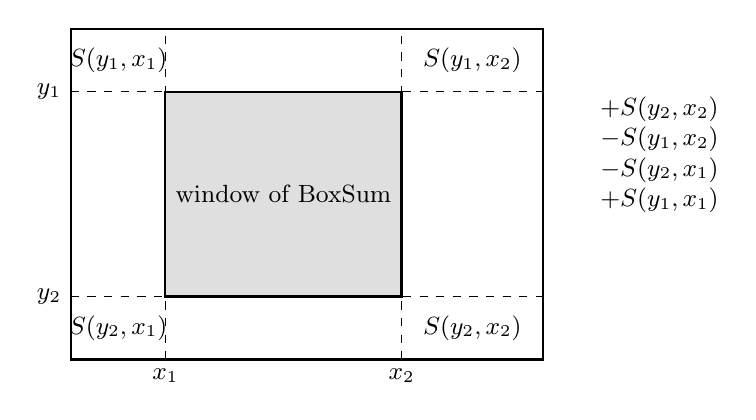
\begin{tikzpicture}[x=1cm,y=1cm]
\fill[gray!25] (1.2,0.8) rectangle (4.2,3.4);
\draw[thick] (0,0) rectangle (6,4.2);
\draw[thick] (1.2,0.8) rectangle (4.2,3.4);
\foreach \x/\l in {1.2/{$x_1$},4.2/{$x_2$}} {\draw[dashed] (\x,0) -- (\x,4.2); \node[font=\small,below] at (\x,0) {\l};}
\foreach \y/\l in {0.8/{$y_2$},3.4/{$y_1$}} {\draw[dashed] (0,\y) -- (6,\y); \node[font=\small,left] at (0,\y) {\l};}
\node[font=\small] at (2.7,2.1) {window of $\mathrm{BoxSum}$};
\node[font=\small] at (0.6,3.8) {$S(y_1,x_1)$};
\node[font=\small] at (5.1,3.8) {$S(y_1,x_2)$};
\node[font=\small] at (0.6,0.4) {$S(y_2,x_1)$};
\node[font=\small] at (5.1,0.4) {$S(y_2,x_2)$};
\node[font=\small,align=left,anchor=west] at (6.6,2.6) {$+S(y_2,x_2)$\\$-S(y_1,x_2)$\\$-S(y_2,x_1)$\\$+S(y_1,x_1)$};
\end{tikzpicture}
\caption{The four-corner rule of the summed-area table. Each table entry $S(y,x)$ is the sum of all pixels above and to the left of $(y,x)$ (measured with the vertical axis pointing down), so the shaded window sum follows from four entries (Equation~\ref{eq:seg-boxsum}).}
\label{fig:seg-boxsum}
\end{figure}

\figplaceholder{5.2cm}{Four panels of the same photograph: (a) colour photograph resized to 2400 px; (b) luma grey image $G$; (c) background estimate $B$ as a heat map; (d) corrected image $I_{\mathrm c}$. Source: run the stages of \texttt{ProcessPage} on a personal page, e.g. \texttt{NOGIT/dylan/preprocessing\_deskew\_ruleline\_border\_cleanup.jpg}, and save the intermediate arrays.}
\caption{Illumination correction. The estimated background (c) follows the lighting gradient of the photograph, and its division from the grey image yields a flat white paper level (d) on which a local threshold is reliable.}
\label{fig:seg-illum}

\figplaceholder{4.6cm}{Page-mask construction as a $2\times3$ panel: Otsu paper candidates, largest component, hole-filled and closed mask, convex-hull notch repair, final eroded mask overlaid on the photograph. Source: stage~2 of \texttt{ProcessPage}.}
\captionof{figure}{Construction of the page mask (placeholder).}
\label{fig:seg-mask}

\begin{figure}[h]
\centering
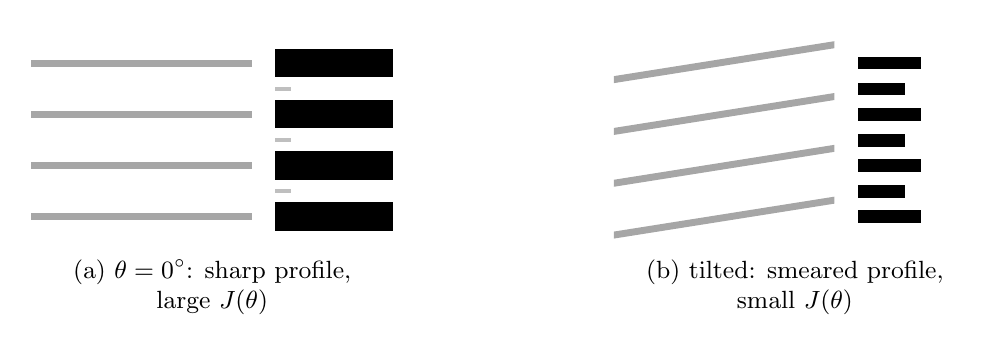
\begin{tikzpicture}[x=1cm,y=1cm]
% left: aligned lines
\begin{scope}
\foreach \k in {0,1,2,3} {\draw[line width=2.5pt,gray!70] (0,\k*0.65) -- (2.8,\k*0.65);}
\foreach \k in {0,1,2,3} {\fill[black] (3.1,\k*0.65-0.18) rectangle (3.1+1.5,\k*0.65+0.18);}
\foreach \k in {0,1,2} {\fill[black!25] (3.1,\k*0.65+0.3) rectangle (3.1+0.2,\k*0.65+0.35);}
\node[font=\small,align=center] at (2.3,-0.9) {(a) $\theta=0^\circ$: sharp profile,\\ large $J(\theta)$};
\end{scope}
% right: tilted lines
\begin{scope}[xshift=7.4cm]
\begin{scope}
\clip (0,-0.4) rectangle (2.8,2.4);
\foreach \k in {0,1,2,3} {\draw[line width=2.5pt,gray!70,rotate around={9:(1.4,1.0)}] (-0.4,\k*0.65) -- (3.2,\k*0.65);}
\end{scope}
\foreach \k in {0,1,2,3} {\fill[black] (3.1,\k*0.65-0.08) rectangle (3.1+0.8,\k*0.65+0.08);}
\foreach \k in {0,1,2} {\fill[black] (3.1,\k*0.65+0.24) rectangle (3.1+0.6,\k*0.65+0.40);}
\node[font=\small,align=center] at (2.3,-0.9) {(b) tilted: smeared profile,\\ small $J(\theta)$};
\end{scope}
\end{tikzpicture}
\caption{Principle of the projection-variance skew search. The bars on the right of each panel represent the row-sum profile of the ink. Aligned lines (a) give strong peaks and empty gaps and therefore a large variance, whereas a tilt (b) fills the gaps.}
\label{fig:seg-skew}
\end{figure}

\figplaceholder{4.4cm}{Skew search on a deliberately tilted photograph: left, plot of $J(\theta)$ for the coarse and fine grids with the chosen angle marked; right, the page before and after rotation with the angle. Source: call the skew estimator with each candidate angle and store the scores.}
\captionof{figure}{Measured skew-search objective $J(\theta)$ (placeholder).}
\label{fig:seg-skewmeas}

\begin{figure}[h]
\centering
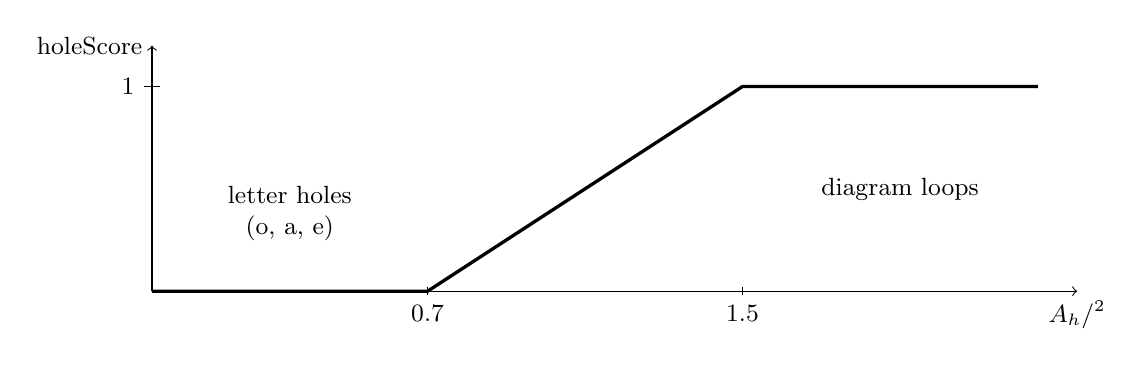
\begin{tikzpicture}[x=5cm,y=2.6cm]
\draw[->] (0,0) -- (2.35,0) node[below,font=\small] {$A_h/\wht^2$};
\draw[->] (0,0) -- (0,1.2) node[left,font=\small] {holeScore};
\draw[very thick] (0,0) -- (0.7,0) -- (1.5,1) -- (2.25,1);
\foreach \xx in {0.7,1.5} {\draw (\xx,0.02) -- (\xx,-0.02) node[below,font=\small] {\xx};}
\draw (0.02,1) -- (-0.02,1) node[left,font=\small] {1};
\node[font=\small,align=center] at (0.35,0.38) {letter holes\\(o, a, e)};
\node[font=\small,align=center] at (1.9,0.5) {diagram loops};
\end{tikzpicture}
\caption{Score ramp of Equation~\ref{eq:seg-mess}. Holes that are smaller than $0.7\wht^2$ are treated as letter counters and give a zero score, holes larger than $1.5\wht^2$ give the maximum score.}
\label{fig:seg-ramp}
\end{figure}

\begin{table}[h]
\centering
\fontsize{9.5}{11.5}\selectfont
\begin{tabularx}{\linewidth}{|p{2.6cm}|X|X|}
\hline
\textbf{Decision} & \textbf{Alternative} & \textbf{Reason for the choice} \\
\hline
Ink threshold & Global fixed or Otsu threshold; local mean and standard-deviation threshold & Photographs have shading of the same order as the ink contrast; division by a blurred background followed by a local mean with offset removes multiplicative and additive variation cheaply. \\
\hline
Blur & Direct Gaussian convolution & Three box means cost $O(1)$ per pixel for any radius with a summed-area table. \\
\hline
Lines & Row projection with gap detection & A projection needs horizontal lines over the full width and cannot separate diagrams; chaining with a baseline curve follows drifting baselines and tags text and non-text. \\
\hline
Skew & Hough transform of edges & Edge directions are dominated by rules and diagrams; the projection variance matches the row grouping that follows. \\
\hline
Rule removal & Long morphological opening & An opening erases long underlines and cross-bars and cannot follow a slope; run-length chaining with a page-crossing requirement protects handwriting. \\
\hline
Faint filtering & Fixed darkness cut-off & Pen pressure and lighting differ per page; Otsu on the component darkness calibrates itself. \\
\hline
Text versus diagram & Learned layout detector & Outside the own first-principles scope and unnecessary for the pages of this project. \\
\hline
Page geometry & Four-point perspective warp & Not implemented; the camera looks straight down at the page, so keystone is small. \\
\hline
\end{tabularx}
\caption{Design alternatives of the segmentation block.}
\label{tab:seg-alt}
\end{table}

\paragraph{Stage 2 details.}
The mask is built in ten steps.
\begin{enumerate}
\item A grey image $G_b$ blurred with nominal scale 4 and the saturation of the hue--saturation--value (HSV) colour model, $S=255(\max_c-\min_c)/\max_c$ (maximum and minimum over the colour channels) are computed.
\item A global threshold $t^*$ is found by the method of Otsu \cite{otsu1979}, which maximises the between-class variance of the intensity histogram,
(equation as in the main text)
where $\omega_B(t)$ and $\omega_F(t)$ are the numbers of pixels below and above $t$, and $\mu_B(t)$ and $\mu_F(t)$ the mean intensities of the two classes (the normalisation $1/N^2$ is omitted because it does not change the arg max).
A global threshold is appropriate here because the paper--desk contrast is large.
\item The candidate set ``paperish'' is $\{G_b\ge t^*\}\wedge\{S<90\}$ (paper is bright and has low saturation); it is opened with a $9\times9$ square and only the largest 4-connected component is kept.
\item To admit parts of the sheet that lie in shadow, the threshold is re-derived from the paper itself: with $m_p$ the median of $G_b$ over the current mask, the set $\{G_b\ge m_p-50\}\wedge\{S<90\}$ is opened and its largest component kept.
\item Holes are filled (background components that do not touch the frame border), the mask is closed with a $15\times15$ square, and holes are filled again.
\item Ragged protrusions (fingers, shadows) are trimmed by a profile test on each axis: with $p$ the mask-sum profile, only samples with $p\ge 0.30\,\mathrm{median}(p\,|\,p>0.2\max p)$ are kept and the largest contiguous run is retained. The factor 0.30 is deliberately low so that a page that is cut off by the frame is not trimmed.
\item Rows and columns darker than the cut level of Equation~\ref{eq:seg-dark}
\begin{equation}
c=\min\!\bigl(m_p-45,\;\max(m_p-85,\;\tfrac12(m_p+m_{bg}))\bigr)
\label{eq:seg-dark}
\end{equation}
are trimmed, where $m_p$ is the median blurred brightness inside the mask and $m_{bg}$ that outside; a page edge in soft shadow (about 0.7 of the paper brightness) is still far brighter than the desk, so the cut level is placed relative to what actually lies off the page.
\item \emph{Shadow-notch repair.} A photographed sheet is a convex quadrilateral, so a concave notch in the mask is a shadow artefact. Each column and row of the mask is made contiguous between its first and last mask pixel, the convex hull of the result is filled, and new pixels are accepted only if $G_b\ge0.55\,m_p$; holes are then filled again.
\item The mask is eroded by a square of odd side $k=2\lfloor e/2\rfloor+1$ with $e=\max(4,\lfloor0.006\min(H,W)\rfloor)$ (about 11 pixels), so that the paper edge itself is not binarised as ink.
\item If the mask covers less than 15\,\% of the frame or no component exists, the mask is set to the whole frame, because abandoning page detection is safer than losing the page.
\end{enumerate}
The method fails for strongly tinted paper (saturation above 90), when the desk is almost as bright as the paper, or when the sheet violates the convexity assumption, and the fallback then applies. Figure~\ref{fig:seg-mask} is reserved for an example of the construction of the mask.


\paragraph{Stage 6 details.}

Ruled paper and other printed structure joins words and lines into giant components, so these structures must be removed \emph{without} removing handwriting that touches them.
Four removal steps are applied in sequence; each is rule-aware or scale-aware so that they act only on components that cannot be handwriting.

\paragraph{Rules by run lengths and chaining.}
For each ink pixel $p$ the length $h\mathrm{Run}(p)$ of its horizontal run and $v\mathrm{Run}(p)$ of its vertical run are computed (the runs are computed for all pixels at once from the row differences).
A minimum rule length $L_r=\max(50,\lfloor3.5\wht\rfloor)$ is defined, the rule thickness is the median vertical run $T=\mathrm{median}(v\mathrm{Run}\,|\,h\mathrm{Run}\ge L_r)$ (2 pixels if none exists), and the thickness cut is $\kappa=\max(4,\lfloor1.8T\rfloor)$.
Horizontal rule fragments (Equation~\ref{eq:seg-cand}) are the pixels
\begin{equation}
\mathrm{cand}_H=\bigl(h\mathrm{Run}\ge\max(20,\lfloor0.8\wht\rfloor)\bigr)\wedge\bigl(v\mathrm{Run}\le\kappa\bigr),
\label{eq:seg-cand}
\end{equation}
and vertical candidates are defined symmetrically.
A rule that is broken by crossing strokes or slightly sloped is not one long run, so fragments are chained: the candidate mask is labelled, the components are sorted by $x$, and two components $a$ and $b$ are united if their gap $g=x_b-(x_a+w_a)\le2.5\wht$, their vertical offset satisfies the condition of Equation~\ref{eq:seg-slope}
\begin{equation}
|c_{y,b}-c_{y,a}|\le\Delta_{\max}=2\kappa+0.08\max(0,g)+0.04\,(w_a+w_b),
\label{eq:seg-slope}
\end{equation}
and their darkness differs by at most 55 grey levels ($c_y$ is the centroid row, $w$ the component width, and the allowance grows with the distance so that gentle slope and wobble are tolerated).
A group is declared a rule only if it spans at least $0.6W$ (vertical rules: $0.45H$) and reaches both ends of the page, $x_1\le0.15W$ and $x_2\ge0.85W$ (vertical: $0.2H$ and $0.8H$).
A long word or underline cannot satisfy this condition.
The rule mask is the union dilated by $3\times3$, restricted to pixels with $v\mathrm{Run}\le\kappa+2$ or $h\mathrm{Run}\le\kappa+2$ so that thick pen strokes that cross the rule are not deleted.
Two passes are run, the second catching rules that were hidden behind the first layer or split.
An elongated underline is not a rule: a component is \emph{underline-like} if its width exceeds $4\wht$ and its mean thickness (area over width) is at most 6.5 pixels.

\paragraph{Faint components, rule-aware.}
Components that are fainter than the handwriting (leftover printed rules, bleed-through, shadows) are identified without a fixed threshold.
Candidates are the components with width $>8\wht$, height between $0.25\wht$ and $8\wht$, fill ratio (area over bounding-box area) below 0.2 and a largest enclosed hole of at most $1.4\wht^2$ (a drawing has holes, a rule network does not).
Because a word may be glued to a faint rule, the rule is cut out first: a column is \emph{thin} if its vertical ink span is at most $\max(6,\lfloor0.35\wht\rfloor)$, and each run of at least $\lfloor2\wht\rfloor$ consecutive thin columns is removed; this test is insensitive to the slope of a rule.
For each remaining component the darkness of Equation~\ref{eq:seg-dark2}
\begin{equation}
d=255-P_{25}\bigl(I_{\mathrm c}\,\big|\,\text{component}\bigr)
\label{eq:seg-dark2}
\end{equation}
is computed, where $P_{25}$ is the 25th percentile of the corrected intensity inside the component.
If the 90th and 10th percentiles of $d$ over all components differ by less than 60 the page has no bimodality and nothing is removed; otherwise a one-dimensional Otsu threshold $\tau$ (Equation~\ref{eq:seg-otsu} on 64 histogram bins of $d$) separates faint from normal components, and components with $d<\tau$ are removed, unless $\tau$ lies outside $(P_{10},P_{90})$.
The page therefore defines for itself what ``faint'' means, which suits the differences in pen pressure and lighting between pages; an earlier fixed darkness filter was replaced because it removed words together with the faint rule.
Components that were removed here are re-attached later if they lie on a text line (stage 8).

\paragraph{Page edges and facing pages.}
Junk that touches the left or right edge of the page mask or a corner of it (binding shadows, edge noise) is removed: with $t_x=\max(8,\lfloor0.75\wht\rfloor)$ and $t_c=\lfloor2\wht\rfloor$, a component is removed if it is narrower than $0.15W$ and touches a side edge within $t_x$, or if it touches a side edge and a top or bottom edge within $t_c$ while being narrower than $0.25W$ and lower than $3\wht$.
Ink of a facing page that appears at the image border is found from the column ink profile $c(x)$: after smoothing with a box of width $\max(5,\lfloor\wht\rfloor)$ (made odd), columns above $0.25$ times the median of the ``lively'' columns (those above 5\,\% of the maximum) form blocks, the block with the most ink is dominant, and a smaller block that touches the border zone of $2\wht$ is cut away together with half a glyph height of margin; interior blocks such as margin numbers are retained.

\paragraph{Sparse rule networks.}
Sloped or wavy rules are cut into short runs that the test above misses.
For components with width $>6\wht$, height between $1.2\wht$ and $8\wht$, fill ratio below 0.10 and no large hole, the column-span test is applied with the same thin-column definition and run length $\lfloor2\wht\rfloor$.


\paragraph{Grouping details.}
For each chain the points $(c_x,c_y,A)$, sorted by $x$, give a baseline curve whose ordinate is smoothed by an area-weighted average over a five-point window (Equation~\ref{eq:seg-curve}),
(equation as in the main text)
where $y_k$ and $A_k$ are the centroid row and area of the $k$th point (the window is truncated at the ends), and the curve $y_{\mathrm{curve}}(x)$ is linearly interpolated between the points and constant beyond the ends.
Chains of one physical row are merged in three passes.
\emph{Pass 1} (same local height): chains sorted by mean curve height are merged when they overlap in $x$ and the mean difference of the two curves sampled at seven equally spaced positions of the overlap is below $0.6\wht$, or, if they do not overlap, when the curves differ by less than $0.55\wht$ at the middle of the gap; after each merge the scan restarts.
\emph{Pass 2} (pitch-aware): the line pitch $p$ is the median of the consecutive chain-centre gaps that exceed $0.5\wht$ (fallback $1.8\wht$), and chains are merged when the mean curve difference is below $0.45\,p$ (overlapping) or $0.4\,p$ (not overlapping).
Letting the threshold scale with the measured line spacing handles writing of varying size without manual tuning.
\emph{Pass 3} demotes weak chains: a chain is \emph{strong} if it has at least three components, or a width of at least $3\wht$ and an area of at least $2\wht^2$, or if no other chain lies within $0.8\,p$; the components of weak chains re-enter in the next step.

\paragraph{Leftover components.}
Every component that is not yet in a chain is assigned according to its shape.
An underline-like component is attached to the chain whose curve lies above it by between $-0.2\wht$ and $1.5\wht$.
A component with $h\le1.8\wht$ (dots, accents, punctuation) joins the nearest chain curve within $1.3\wht$, where the distance is $|y_{\mathrm{curve}}(c_x)-c_y|$ plus 0.15 pixel per pixel that the component lies outside the chain's $x$-span, unless it overlaps a \texttt{MESS} block.
A taller component, typically an ascender or descender that links two rows, is split \emph{pixel-wise}: every pixel goes to the nearest chain within $2.5\wht$, and each chain receives its sub-mask if it has at least 8 pixels, so that one connected stroke can be shared by two lines.
A chain finally becomes a line unless its total area is below $0.35\wht^2$, its tallest component below $0.35\wht$, or it consists of at most three small solid blobs of total width below $3.5\wht$ (stray dots).
Text lines whose bounding box lies more than 70\,\% inside the core box of a \texttt{MESS} block are absorbed into that block, so that labels inside a diagram are not exported as lines.

\paragraph{Refinement.}
A refinement step rejoins a physical row that chaining split, for example because of a word gap larger than $6\wht$.
With cap $\min(0.5\,p,1.6\wht)$, two lines whose centres differ by at most $0.75\,p$ are merged if one of four signals holds: (i)~the centres differ by less than $0.5\wht$; (ii)~their vertical ranges overlap by at least 70\,\% of the shorter range, centres differ by less than $0.45\,p$ and the smaller line has an area below $4\wht^2$; (iii)~they overlap in $x$ by at most 55\,\% of the narrower width and their curves, evaluated at the middle of the overlap, differ by less than the cap; or (iv)~centres differ by less than $0.6\,p$ and less than 30\,\% of the columns of the narrower line are shared with the other (words interleave along $x$, whereas stacked rows always share columns).
Underline-shaped components that lie at least $0.5\wht$ above their line's curve are moved to the line below which they sit, because an underline belongs to the text written above it, and pale components that were removed as faint are re-attached to the nearest curve when they lie within $0.75\wht$ of it.
The \texttt{TEXT} and \texttt{MESS} items are finally sorted by their vertical centre; a \texttt{MESS} item that is immediately followed by a \texttt{TEXT} item whose centre falls in the top 40\,\% of the block is swapped with it, so that a caption precedes its diagram.



\subsection{Appendix: Text recogniser (supporting material)}

This part of the appendix contains the supporting figures and tables of Section~\ref{sec:textrec}: the layer table, the LSTM cell, the pre-processing schematic, the data sets, the training stages, the forgetting experiment, the alternatives and the details of the inference implementation.

\begin{figure}[h]
\centering
\begin{tikzpicture}[x=1cm,y=1cm]
\draw[thick,fill=gray!15] (0,2.2) rectangle (5.6,3.3);
\node[font=\small] at (2.8,2.75) {line crop: $w\times h$ pixels, variable};
\draw[w2arr] (2.8,2.1) -- (2.8,1.4) node[midway,right,font=\small] {scale by $s$, Equation~\ref{eq:rec-resize}};
\draw[thick] (0,0) rectangle (8,0.8);
\draw[thick,fill=gray!15] (0,0.1) rectangle (5.6,0.7);
\node[font=\small] at (2.8,0.4) {scaled line $w'\times h'$};
\node[font=\small] at (6.8,0.4) {white padding};
\node[font=\small,anchor=east] at (-0.1,0.4) {64};
\node[font=\small,anchor=north] at (4,-0.05) {640 pixels};
\draw[<->] (-0.05,0) -- (-0.05,0.8);
\node[font=\small,align=left,anchor=west] at (8.5,0.4) {ink $\rightarrow+1$\\ paper $\rightarrow-1$};
\end{tikzpicture}
\caption{Pre-processing of a line crop. The crop is scaled uniformly, left-aligned on a white canvas and normalised to the range $[-1,1]$ (Equation~\ref{eq:rec-norm}).}
\label{fig:rec-canvas}
\end{figure}

\begin{table}[h]
\centering
\fontsize{9.5}{11.5}\selectfont
\begin{tabular}{|l|l|r|}
\hline
\textbf{Layer} & \textbf{Output shape} & \textbf{Trainable parameters} \\
\hline
Input & $1\times64\times640$ & 0 \\
Conv 3$\times$3 (1$\to$32), BN, ReLU & $32\times64\times640$ & 384 \\
Conv 3$\times$3 (32$\to$32), BN, ReLU & $32\times64\times640$ & 9\,312 \\
Max-pool 2$\times$2 & $32\times32\times320$ & 0 \\
Conv 3$\times$3 (32$\to$64), BN, ReLU & $64\times32\times320$ & 18\,624 \\
3$\times$ Conv 3$\times$3 (64$\to$64), BN, ReLU & $64\times32\times320$ & 111\,168 \\
Max-pool 2$\times$2 & $64\times16\times160$ & 0 \\
Conv 3$\times$3 (64$\to$128), BN, ReLU & $128\times16\times160$ & 74\,112 \\
5$\times$ Conv 3$\times$3 (128$\to$128), BN, ReLU & $128\times16\times160$ & 739\,200 \\
Height max-pool & $128\times1\times160$ & 0 \\
BiLSTM layer 1 (128$\to$256, 2 directions) & $160\times512$ & 790\,528 \\
BiLSTM layer 2 (512$\to$256, 2 directions) & $160\times512$ & 1\,576\,960 \\
Linear (512$\to$75) & $160\times75$ & 38\,475 \\
Log-softmax & $160\times75$ & 0 \\
\hline
\textbf{Total} & & \textbf{3\,358\,763} \\
\hline
\end{tabular}
\caption{Layer-by-layer shapes and trainable parameters of the text recogniser (batch dimension omitted). Batch normalisation also stores 2\,176 non-trainable running statistics, and the checkpoint therefore holds 3\,360\,951 numbers (13.4\,MB as 32-bit floating point).}
\label{tab:rec-layers}
\end{table}

\begin{figure}[h]
\centering
\begin{tikzpicture}[x=1cm,y=1cm]
\draw[thick,rounded corners=3pt] (0,0) rectangle (8,3.6);
\node[w2box,minimum width=1cm] (f) at (1.4,1.2) {$\sigma$};
\node[w2box,minimum width=1cm] (i) at (3.0,1.2) {$\sigma$};
\node[w2box,minimum width=1cm] (g) at (4.6,1.2) {$\tanh$};
\node[w2box,minimum width=1cm] (o) at (6.6,1.2) {$\sigma$};
\node[font=\scriptsize] at (1.4,0.55) {$f_t$};
\node[font=\scriptsize] at (3.0,0.55) {$i_t$};
\node[font=\scriptsize] at (4.6,0.55) {$g_t$};
\node[font=\scriptsize] at (6.6,0.55) {$o_t$};
\draw[thick,-{Stealth}] (-0.8,3.0) -- (8.8,3.0) node[right,font=\small] {$c_t$};
\node[font=\small,left] at (-0.8,3.0) {$c_{t-1}$};
\node[w2dark,circle,inner sep=1pt] (m1) at (1.4,3.0) {$\odot$};
\node[w2dark,circle,inner sep=1pt] (a1) at (3.8,3.0) {$+$};
\node[w2dark,circle,inner sep=1pt] (m2) at (3.8,2.1) {$\odot$};
\node[w2box,minimum width=0.9cm] (th) at (6.6,3.0) {$\tanh$};
\node[w2dark,circle,inner sep=1pt] (m3) at (6.6,2.1) {$\odot$};
\draw[w2arr] (f) -- (m1);
\draw[w2arr] (i) |- (m2); \draw[w2arr] (g) |- (m2); \draw[w2arr] (m2) -- (a1);
\draw[w2arr] (o) -- (m3); \draw[w2arr] (th) -- (m3);
\draw[w2arr] (m3) -- ++(0,-2.6) -- ++(0,0);
\node[font=\small,anchor=west] at (7.0,2.1) {$h_t$};
\node[font=\small,anchor=north] at (4.0,-0.2) {inputs of all four gates: $[x_t,\,h_{t-1}]$};
\end{tikzpicture}
\caption{Schematic of an LSTM cell (Equation~\ref{eq:rec-lstm}). The memory line $c_t$ at the top is changed only by the forget gate (multiplication) and the input gate (addition), which allows information to travel over many time steps.}
\label{fig:rec-lstm}
\end{figure}

\begin{table}[h]
\centering
\fontsize{9.5}{11.5}\selectfont
\begin{tabularx}{\linewidth}{|p{2.8cm}|p{3.6cm}|X|}
\hline
\textbf{Data set} & \textbf{Split rule} & \textbf{Caveat on the validation figure} \\
\hline
Lines segmented by the student's own block from scanned database pages, with labels generated by alignment (first stage only) &
The last labelled page of every writer is held out. &
Same writers in training and hold-out, so the figure is writer-dependent; the labels are project-generated and noisy. \\
\hline
Public line-level IAM transcription set: 6\,482 training, 976 validation, 2\,915 test lines (6\,481, 976 and 2\,915 after label cleaning) &
Official training, validation and test partitions. &
The validation set drives learning-rate decay and checkpoint choice, so its accuracy is mildly optimistic; the test set is used for no decision. The partitions are believed, but not verified, to be writer-independent, and the warm start from the first stage may have seen some of the same forms. \\
\hline
13 photographed pages of the two personal writers (8 and 5 pages), 355 transcription lines of which one is a diagram marker &
Per page, 15\,\% of the lines (at least one) are drawn at random with a fixed seed as validation; about 52 validation lines in total. &
Validation lines come from the same pages, pen, paper, lighting and vocabulary as training lines; the figure measures ``same writer, same notebook, new lines'' and is optimistic. It also takes part in checkpoint selection. \\
\hline
Ten-author hold-out (eight database writers and the two personal writers) &
Used only as an evaluation set. &
The held-out database lines may have been seen in the line-level training data, and their labels are project-generated, so the figure is not a writer-independent measure. \\
\hline
\end{tabularx}
\caption{Data sets of the text recogniser and their leakage assessment.}
\label{tab:rec-data}
\end{table}

\begin{table}[h]
\centering
\fontsize{9.5}{11.5}\selectfont
\begin{tabularx}{\linewidth}{|l|l|l|l|l|l|X|}
\hline
\textbf{Stage} & \textbf{Data} & \textbf{$\eta_0$} & \textbf{Batch} & \textbf{Epochs} & \textbf{Clip} & \textbf{Schedule and selection} \\
\hline
Base & own lines & $10^{-3}$ & 16 & $\le200$ & none & halve after 5 stalls; stop after 15; up to 3 restarts from the best weights; best validation loss \\
\hline
Clean labels & public set & $10^{-3}$ & 16 & $\le200$ & none & as above, up to 8 restarts; best public validation loss \\
\hline
Personal & personal lines & $3\!\times\!10^{-4}$ & 8 & 60 & 5 & halve after 5 stalls; best personal validation loss \\
\hline
Joint & both, $f=0.20$ & $5\!\times\!10^{-4}$ & 16 & 30 & 5 & halve after 4 stalls on the sum of both validation losses; best $\min$ of the two accuracies \\
\hline
\end{tabularx}
\caption{Hyper-parameters of the four training stages. All stages use RMSprop (Equation~\ref{eq:rec-rmsprop}) with weight decay $10^{-5}$; the minimum learning rate was $10^{-5}$ or $10^{-6}$.}
\label{tab:rec-stages}
\end{table}

\begin{table}[h]
\centering
\fontsize{9.5}{11.5}\selectfont
\begin{tabular}{|l|r|r|r|}
\hline
\textbf{Training} & \textbf{Public val./test (\%)} & \textbf{Personal val. (\%)} & \textbf{Remark} \\
\hline
Clean-label stage only & 93.87 / 91.60 & -- & before personal data \\
Personal only, all layers & 84.26 / 80.56 & 90.2 & forgetting \\
Personal only, frozen convolutions & 85.87 / 82.62 & 88.5 & forgetting \\
Joint (deployed) & 94.03 / 91.82 & 89.64 & both domains kept \\
\hline
\end{tabular}
\caption{The catastrophic-forgetting experiment: character accuracies of the three ways of adding personal data.}
\label{tab:rec-forget}
\end{table}

\begin{table}[h]
\centering
\fontsize{9.5}{11.5}\selectfont
\begin{tabularx}{\linewidth}{|p{3.2cm}|X|X|}
\hline
\textbf{Alternative} & \textbf{For} & \textbf{Against} \\
\hline
Character segmentation and a per-character classifier (small convolutional network) &
Simple network; the proposal's plan. &
Needs a segmenter that works on joined letters; classification errors cannot be repaired by context; needs character-level labels that the available data lack. \\
\hline
Line-level CNN-BiLSTM-CTC (chosen) &
No segmentation below the line; alignment-free training from line transcriptions; context from both sides; output is a string; 3.36 million parameters can be run by a from-scratch implementation. &
Needs line segmentation; greedy decoding leaves spelling errors; CTC assumes independent steps. \\
\hline
Lexicon or language-model decoding &
Repairs near-miss words; gives the lowest error in the published design. &
Needs a corpus and a decoder; the technical vocabulary and symbols of the pages are largely out of vocabulary. Future work. \\
\hline
Deeper backbones with skip connections &
Easier training of very deep networks. &
The 12-layer network with batch normalisation trained well; larger models cost memory and time on the single-board computer. \\
\hline
Attention-based encoder--decoder or transformer &
Strong accuracy on large corpora. &
Far more parameters, large pre-training data, slow autoregressive decoding that can skip or invent text, and hard to implement from scratch for the board. \\
\hline
Word-level recognition &
Uses the lexicon directly. &
Needs word segmentation and a closed vocabulary; poor for names, numbers and symbols. \\
\hline
\end{tabularx}
\caption{Alternatives to the line-level recogniser.}
\label{tab:rec-alt}
\end{table}

\paragraph{Text recogniser: weight file and inference details.}

Training needs a large software environment, which should not be installed on the single-board computer.
The student therefore wrote a separate, from-scratch inference implementation in Python that reads the trained weights directly and uses only array arithmetic.
It consists of three small modules (about 480 lines in total): the layer functions, the network, and a weight reader.

\paragraph{Convolution as a matrix product.}
Each convolution is converted to one matrix multiplication (the im2col method).
The padded input is cut into overlapping $3\times3$ patches, and every patch is flattened into one column of a matrix $\mathrm{cols}\in\mathbb R^{(C_{\mathrm{in}}k^2)\times(H_{\mathrm{out}}W_{\mathrm{out}})}$; with the weights reshaped to $\tilde W\in\mathbb R^{C_{\mathrm{out}}\times C_{\mathrm{in}}k^2}$,
(equation as in the main text)
where $b\,\mathbf 1^\top$ adds the bias of each output channel to all positions.
In Equation~\ref{eq:rec-im2col}, one optimised matrix product replaces the six nested loops of Equation~\ref{eq:rec-conv} and was found to be about ten times faster than a general summation routine, with a difference of about $10^{-13}$ between the two.
The cost is memory: the largest matrix, for the second convolution of stage 1, has $288\times40\,960$ entries (47\,MB as 32-bit floating point), and the largest activation tensor is 5.2\,MB, so the working set is a few tens of megabytes.
Batch normalisation is applied in its folded form of Equation~\ref{eq:rec-bnfold}, pooling uses windowed views of the array, the height collapse is a maximum over one axis, and the LSTM is an explicit loop over the 160 steps with one product of $1024$ rows per step and direction, the backward direction being a pass over the reversed sequence.

\paragraph{Reading the trained weights.}
The training-time weight file is an archive that contains a serialised object structure, in which every tensor is replaced by a reference to a storage key, and one raw little-endian byte file per storage.
The student's weight reader opens the archive, parses the object structure with a customised reader that intercepts the tensor and storage constructors, reads the bytes of each storage into an array, rebuilds every tensor from its shape and strides, and returns a dictionary of 102 arrays with the names of the training model.
The inference code then indexes the weights by name, and no machine-learning software is needed at run time.

\paragraph{Agreement with the training code and cost.}
For one random $64\times640$ input, the largest difference between the $160\times75$ log-probability matrices of the inference code and the training code was $2.3\times10^{-5}$ for the deployed weights, $1.1\times10^{-5}$ for the clean-label stage and $9.5\times10^{-6}$ for the personal stage, with identical arg-max (and therefore decoded text) at all 160 steps; this is a single synthetic input and not a test-set sweep.
The weights occupy 13.4\,MB.
On the development computer (processor only) one forward pass of one line took 2.6 to 3.1\,s; for a line of 40 characters this is about 65 to 75\,ms per character, which exceeds the 25\,ms per character that requirement R4 allows, and the ARM processor of the single-board computer is expected to be slower.
\textbf{[TO BE COMPLETED BY STUDENT: measure the recognition time per line on the ODROID N2+; the project files contain no such measurement, and the proposal's budget may refer to the whole classification step.]}
Optional compiled replacements for the convolution and the LSTM exist but are not used: the compiled convolution was slower than the optimised matrix product on a desktop processor, and the compiled LSTM was 2.8 to 4.4 times faster than the array version.



\subsection{Appendix: Writer identification (supporting material)}

This part of the appendix contains the layer table, the data and training tables, the real stroke-normalisation example and the aggregation diagram of Section~\ref{sec:writerid}.

\begin{table}[h]
\centering
\fontsize{9.5}{11.5}\selectfont
\begin{tabular}{|l|l|r|}
\hline
\textbf{Block} & \textbf{Output shape} & \textbf{Trainable parameters} \\
\hline
Stage 1 (2 conv units, 32 channels) & $32\times64\times640$ & 9\,696 \\
Max-pool 2$\times$2 & $32\times32\times320$ & 0 \\
Stage 2 (4 conv units, 64 channels) & $64\times32\times320$ & 129\,792 \\
Max-pool 2$\times$2 & $64\times16\times160$ & 0 \\
Stage 3 (6 conv units, 128 channels) & $128\times16\times160$ & 813\,312 \\
Height max-pool and width mean-pool & 128 & 0 \\
FC 128$\to$96, ReLU, dropout & 96 & 12\,384 \\
FC 96$\to$10 & 10 & 970 \\
\hline
\textbf{Total} (backbone 952\,800, head 13\,354) & & \textbf{966\,154} \\
\hline
\end{tabular}
\caption{Layer shapes and parameters of the writer classifiers. Batch normalisation adds 2\,176 non-trainable running statistics (968\,330 stored numbers in total), and a forward pass needs about $3.79\times10^9$ multiply--accumulate operations.}
\label{tab:wid-layers}
\end{table}

\begin{table}[h]
\centering
\fontsize{9.5}{11.5}\selectfont
\begin{tabular}{|l|r|r|l|}
\hline
\textbf{Writer} & \textbf{Training lines} & \textbf{Validation lines} & \textbf{Validation lines are} \\
\hline
150, 151, 152, 153 & 82, 78, 79, 88 & 9, 8, 8, 9 & the held-out page \\
384, 551, 552, 588 & 72, 78, 63, 78 & 11, 8, 10, 8 & the held-out page \\
Personal writer 1 & 118 & 20 & random lines of training pages \\
Personal writer 2 & 184 & 32 & random lines of training pages \\
\hline
\textbf{Total} & \textbf{920} & \textbf{123} & \\
\hline
\end{tabular}
\caption{Lines of the shape classifier. The ink classifier uses the same split but its counts may differ slightly, because no lines are lost to the stroke normalisation.}
\label{tab:wid-data}
\end{table}

\begin{table}[h]
\centering
\fontsize{9.5}{11.5}\selectfont
\begin{tabular}{|l|l|l|}
\hline
& \textbf{Ink classifier} & \textbf{Shape classifier} \\
\hline
Optimiser, weight decay & AdamW, $10^{-4}$ & AdamW, $10^{-4}$ \\
Initial learning rate & $10^{-3}$ & $3\times10^{-3}$ \\
Schedule & cosine over the epochs & cosine over 500 epochs \\
Epochs & 20 (default) & 500 \\
Batch & 16 images & 64 feature vectors \\
Gradient clipping & global norm 5 & none \\
Trainable parameters & 966\,154 & 13\,354 \\
Checkpoint rule & best validation accuracy & best validation accuracy \\
\hline
\end{tabular}
\caption{Training settings of the two writer classifiers. The best epoch and the number of epochs that were actually run for the stored weights were not recorded.}
\label{tab:wid-hyper}
\end{table}

\figplaceholder{4.6cm}{Real example of the stroke normalisation on one line from one database writer and one personal writer: grey crop, Otsu mask with rules removed, core band with $x_h$, Zhang--Suen skeleton, re-inked line, final canvas. Source: apply the stroke-normalisation function to crops from \texttt{Data/Datasets/IAMpages10} and \texttt{Software/CNN/NOGIT/dylan}.}
\captionof{figure}{Stroke normalisation of real lines (placeholder).}
\label{fig:wid-strokereal}

\begin{figure}[h]
\centering
\begin{tikzpicture}[x=1cm,y=1cm]
\tikzset{ab/.style={w2box,text width=2.5cm,minimum height=1.2cm}}
\node[ab] (a) at (-5.6,0) {$N$ text-line crops from segmentation};
\node[ab] (b) at (-2.8,0) {ink classifier for each line: $p^{(1)},\ldots,p^{(N)}$};
\node[ab] (c) at (0,0) {mean $\bar p$ (Equation~\ref{eq:wid-aggr})};
\node[ab] (d) at (2.8,0) {arg-max: writer $\hat k$};
\node[ab] (e) at (5.6,0) {confidence $100\,\bar p_{\hat k}$ and all $\bar p_k$ to browser};
\foreach \p/\q in {a/b,b/c,c/d,d/e} \draw[w2arr] (\p)--(\q);
\end{tikzpicture}
\caption{Aggregation of line decisions to a page decision in the classification mode.}
\label{fig:wid-aggr}
\end{figure}

\begin{table}[h]
\centering
\fontsize{9.5}{11.5}\selectfont
\begin{tabularx}{\linewidth}{|p{3.4cm}|X|X|}
\hline
\textbf{Alternative} & \textbf{For} & \textbf{Against} \\
\hline
Hand-crafted features (slant, x-height, spacing, connectedness) with nearest-profile classification &
Interpretable; the style-profile builder already measures these features. &
Needs feature selection; weak when two hands are similar in coarse statistics (writer 150 and a personal writer); no classification accuracy of such a method was measured. \\
\hline
Contour-direction and allograph statistics \cite{bulacu2007} &
Text-independent and strong for large writer sets. &
Hand-built features; less direct as a judge of constant-width output. \\
\hline
Siamese or metric learning &
Open-set: new writers without retraining. &
Needs pair mining and threshold calibration; the project needs only a closed set of ten. \\
\hline
Deep fragment or patch networks \cite{he2020} &
Scale to hundreds of writers. &
Only ten writers and about 1\,000 lines are available. \\
\hline
One joint network with a text head and a writer head &
A single backbone. &
Tried first: writer accuracy reached 98.9 to 100\,\% by epoch 20 while the text accuracy stalled at 28 to 29\,\%, so separate single-task networks were adopted. \\
\hline
Ink classifier with random pen-width augmentation &
No second network. &
Reduces but does not remove the thickness cue; the normalisation removes it by construction and matches the transform of the plotter. No ablation was run. \\
\hline
\end{tabularx}
\caption{Alternatives to the two-classifier design.}
\label{tab:wid-alt}
\end{table}


\subsection{Appendix: Relation of the implemented blocks to the proposal}

Table~\ref{tab:des-fumap} relates every implemented block to the functional units of the project proposal (see Section~\ref{sec:blockdiagram}).

\begin{table}[h]
\centering
\fontsize{9.5}{11.5}\selectfont
\begin{tabularx}{\linewidth}{|p{1.5cm}|X|X|}
\hline
\textbf{Proposal unit} & \textbf{Implemented block} & \textbf{Difference and reason} \\
\hline
FU 1.1, 1.2 & USB camera over an A4 page, read by the operating-system driver. & As planned; the ``serial bitstream converter'' is the standard camera interface. \\
\hline
FU 2.1 & Page conditioning (Section~\ref{sec:segmentation}). & Much larger than planned: lighting, skew, ruled paper, neighbouring pages and diagrams are handled. \\
\hline
FU 2.2 & Line segmentation (Section~\ref{sec:segmentation}). & Lines instead of characters, because cursive characters have no reliable boundaries. \\
\hline
FU 2.3 & Text recogniser and writer classifier (Sections~\ref{sec:textrec} and~\ref{sec:writerid}). & Two separate networks instead of one character classifier. \\
\hline
FU 2.4 & Offline training programs. & Not on the single-board computer, because training needs far more memory and time than inference. \\
\hline
FU 2.5, 2.6 & Style-profile builder and permanent profile files (Section~\ref{sec:styleprofile}). & Offline; stores letter paths per writer instead of one trajectory per recognised character. \\
\hline
FU 2.7 & Synthesiser (Section~\ref{sec:synthesis}). & Constructs new text from stored letter variants and adds a best-of-$N$ search. \\
\hline
FU 2.8 & G-code generator and interpreter with pulse generation (Sections~\ref{sec:gcode} and~\ref{sec:gantry}). & Split into two stages with a standard interchange format, which allows the trajectory to be checked without the gantry. \\
\hline
FU 3.1 & Stepper driver modules on 3.3\,V pins. & No separate voltage-shifter block is documented. \textbf{[TO BE COMPLETED BY STUDENT: confirm.]} \\
\hline
FU 3.2 & Two stepper motors on one gantry. & As planned. \\
\hline
FU 3.3, 3.4 & Pen holder and toggle pen-lift motor with position switch. & Pen lift is not driven through the stepper driver, as the proposal assumed, but by a one-direction gear motor with feedback switch. \\
\hline
FU 4 & Power supply. & Not documented in the project files. \\
\hline
(new) & End-stop switches and web server. & Added for protection of the mechanism and to replace the proposed display and input interface. \\
\hline
\end{tabularx}
\caption{Relation of the implemented blocks to the functional units of the project proposal.}
\label{tab:des-fumap}
\end{table}


\subsection{Appendix: further details of Sections 3.3 to 3.5}

This part of the appendix collects paragraphs that were condensed in the main text of Sections~\ref{sec:segmentation} and~\ref{sec:textrec}.

\paragraph{Stage 4: why not a global threshold}
\emph{Why not a single global threshold?} Handwriting on a photographed page has a pen--paper contrast of tens of grey levels, and the residual shading has the same order of magnitude, so a single threshold would either drop strokes in dim areas or turn shadows into ink.
A global threshold according to Otsu \cite{otsu1979} is appropriate for flat-bed scans and is used for the database scans (see below) and for the page mask, but not for photographs.
A local threshold that also uses the local standard deviation \cite{sauvola2000} would handle low-contrast empty regions better but requires a second integral image of squared values; the two-step normalisation (division by the background, then a local mean with offset) was found sufficient and is cheaper.


\paragraph{Stage 5: skew limitations and alternatives}
The objective was preferred to a Hough transform of ink edges, because the latter is dominated by ruled lines and diagram strokes, whereas the projection variance is aligned with what grouping needs, namely horizontal rows.
Limitations are that a single global angle is estimated, so page curl and perspective keystone are not corrected, and that a page dominated by a diagram or a double column layout can give a weak optimum.
During development it was found that a sign mismatch between the rotation function and the angle scoring had doubled the skew of every tilted page; the implementation now rotates in the same sense as the scorer, and the search range was widened from $5^\circ$ to $8^\circ$ with the second residual pass. Figure~\ref{fig:seg-skewmeas} is reserved for a measured example of the objective.



\paragraph{Stage 9: crop rendering details}
The recogniser sees only what is in the crop, so rendering decides whether a neighbouring descender or a pale word appears in it.
A pixel-ownership map stores, for every ink pixel, the index of the item that owns it, and a weak component whose strong ink belongs entirely to one item is owned wholly by that item; a neighbouring row's recovery can therefore never take its halo.
The crop of an item is built as follows.
The bounding box of the component pixels is padded by 6 pixels vertically and horizontally by $\max(6,3g)$ with $g=\max(8,\lfloor0.55\wht\rfloor)$.
The component mask is grown by a $3\times3$ dilation, the weak-ink pixels within a $9\times3$ dilation of it are added, and recovery pixels up to $3g$ pixels horizontally are added; all additions exclude pixels owned by another item.
The crop image is white everywhere, and grey values are copied from the darkest evidence $\min(I_{\mathrm c},I_{\mathrm{c,colour}})$ where the mask is true.
Pale words without any strong ink anchor are attached to a text row if they sit on its curve ($|\Delta y|<0.6\wht$), lie within $[x_1-2\wht,\,x_2+12\wht]$ and are at least half as dark as the row's median component; a component of another row is never taken.


\paragraph{Text recogniser: augmentation parameters}
\paragraph{Data augmentation.}
Training images are augmented after the resize to $64\times640$ (never validation images).
Each of four transformations is enabled independently with probability 0.5; if none is enabled the image is unchanged, otherwise one of the enabled ones is chosen uniformly, so that $P(\text{no augmentation})=1/16=6.25\,\%$ and at most one transformation acts on an image.
The transformations are a horizontal \emph{shear} with factor $k\sim U(-0.6,0.6)$ (angle $\arctan k$), a \emph{rotation} by an angle in $U(-2.5^\circ,2.5^\circ)$, an \emph{elastic distortion} \cite{simard2003} in which random displacement fields (uniform in $[-1,1]$ per pixel) are smoothed with a Gaussian of standard deviation $\sigma\in\{3,4\}$ and scaled by $\alpha\in\{15,20\}$ before the image is warped, and a \emph{perspective} distortion in which each corner is moved by up to $d\,W/2$ horizontally and $d\,H/2$ vertically with $d\sim U(0.03,0.08)$.
The fill colour of the geometric transformations is white.
No colour, contrast, noise or blur augmentation and no synthetic pre-training data are used.


The elastic distortion smooths per-pixel random displacements (uniform in $[-1,1]$) with a Gaussian of standard deviation $\sigma\in\{3,4\}$ and scales them by $\alpha\in\{15,20\}$ before warping; the perspective distortion moves each corner by up to $dW/2$ horizontally and $dH/2$ vertically with $d\sim U(0.03,0.08)$; the fill colour is white; there is no colour, contrast, noise or blur augmentation and no synthetic pre-training data.

\subsection{Appendix: further supporting material for Sections 3.3 to 3.5 (second condensation)}

This part of the appendix contains further figures, equations and derivations that were moved out of Sections~\ref{sec:segmentation}, \ref{sec:textrec} and~\ref{sec:writerid}; the equations are those that the main text refers to by number.

\begin{figure}[h]
\centering
\begin{tikzpicture}[x=1cm,y=1cm]
\foreach \x/\y in {0.2/1.3,1.1/1.45,2.0/1.4,3.1/1.55,4.0/1.65,5.2/1.8,6.2/1.9,7.0/2.0} {\draw[fill=gray!35] (\x,\y) rectangle (\x+0.5,\y+0.55);}
\foreach \x/\y in {0.4/0.0,1.4/-0.05,2.3/0.05,3.4/-0.05,4.5/0.0,5.6/0.1} {\draw[fill=gray!35] (\x,\y) rectangle (\x+0.5,\y+0.55);}
\draw[thick,dashed] plot[smooth] coordinates {(0.45,1.55) (1.35,1.7) (2.25,1.67) (3.35,1.82) (4.25,1.92) (5.45,2.07) (6.45,2.17) (7.25,2.27)};
\node[w2lab,anchor=south west] at (0.1,2.15) {baseline curve (line 1)};
\draw[w2arr] (0.7,1.57) -- (1.1,1.72);
\draw[w2arr] (1.6,1.72) -- (2.0,1.68);
\node[w2lab] at (1.65,0.95) {link with cost = gap + $3\Delta y$};
\draw[<->] (2.5,1.0) -- (3.1,1.0);
\node[w2lab,anchor=north] at (2.8,0.98) {gap};
\node[w2lab,anchor=west] at (7.7,1.6) {chain 1};
\node[w2lab,anchor=west] at (6.4,0.25) {chain 2};
\draw[<->] (-0.3,0.28) -- (-0.3,1.57);
\node[w2lab,rotate=90] at (-0.5,0.9) {line pitch $p$};
\end{tikzpicture}
\caption{Schematic of the grouping of components into chains. Boxes are connected components, arrows are links that minimise Equation~\ref{eq:seg-cost}, and the dashed curve is the smoothed baseline of the upper chain.}
\label{fig:seg-chain}
\end{figure}

\paragraph{Weak-ink recovery by hysteresis.}
The strict threshold $C=12$ drops pale strokes, such as a lightly pressed word or blue ink in a dim corner.
If they were added to the structural mask they would create noise components, but if they are omitted from the crop the recogniser sees truncated words.
A weak mask is therefore built with the lower offset $C=3$, and a weak component is accepted when it lies close to strong ink (Equation~\ref{eq:seg-hyst}):
\begin{equation}
\mathrm{result}=\mathrm{strong}\ \vee\ \Bigl(\mathrm{weak}\wedge\bigl[\mathrm{near}\ \vee\ (\mathrm{far}\wedge A\ge40)\bigr]\Bigr),
\label{eq:seg-hyst}
\end{equation}
in which \emph{strong} is the strict ink mask, \emph{near} marks weak components that intersect the strong ink dilated by a $9\times25$ window (vertical radius 4 pixels, horizontal radius 12 pixels), \emph{far} marks weak components that intersect the strong ink dilated horizontally by $\lfloor2\wht\rfloor$ pixels, and $A$ is the component area in pixels.
The vertical window is small so that recovery never bridges two text rows, while the horizontal reach spans a word gap and the area condition lets only substantial pale words (not speckle) in.
The recovery is run on the luma image and on a colour-aware grey image $G_{\mathrm c}=\lfloor0.5\,\mathrm{luma}+0.5\min(R,G,B)\rfloor$, in which blue ink stays dark in a dim corner, and the results are combined.
Thin horizontal pixel runs that are at most 4 pixels thick and at least 10 pixels long are removed from the weak mask so that pale printed rules are not recovered.
The weak mask never influences which components form a line.


\paragraph{Size normalisation.}
The pixel constants of the block (blur radii, minimum component sizes) only have a meaning if every photograph has the same scale, so every photograph is first resampled so that its longer side equals 2400 pixels after the orientation recorded by the camera has been applied.
For a source image $I$ of size $h\times w$ and a target size $h'\times w'$, the value at target pixel $(i,j)$ is obtained by bilinear interpolation at the source position
\begin{equation}
y_s=\frac{(i+0.5)\,h}{h'}-0.5,\qquad x_s=\frac{(j+0.5)\,w}{w'}-0.5,\qquad I'(i,j)=\sum_{a,b\in\{0,1\}}\omega_{ab}\,I(\lfloor y_s\rfloor+a,\lfloor x_s\rfloor+b),
\label{eq:seg-resize}
\end{equation}
where $\omega_{ab}$ are the standard bilinear weights, which are the products of the horizontal and vertical fractional distances to the four neighbouring source pixels, and indices are clamped at the borders.
The colour image is converted to a grey-scale image $G$ with the luma weights of Equation~\ref{eq:seg-luma}
\begin{equation}
G=\mathrm{clip}\,(0.299\,R+0.587\,G_{\mathrm{c}}+0.114\,B,\;0,\;255),
\label{eq:seg-luma}
\end{equation}
in which $R$, $G_{\mathrm c}$ and $B$ are the red, green and blue channels, and $\mathrm{clip}(v,0,255)$ limits $v$ to the range of 8-bit values.
A page that is smaller than 2400 pixels is thereby enlarged and a larger page is reduced; plain bilinear sampling without a pre-filter is used for reduction, which introduces slight aliasing for very large photographs but keeps the operation cheap.


\begin{figure}[h]
\centering
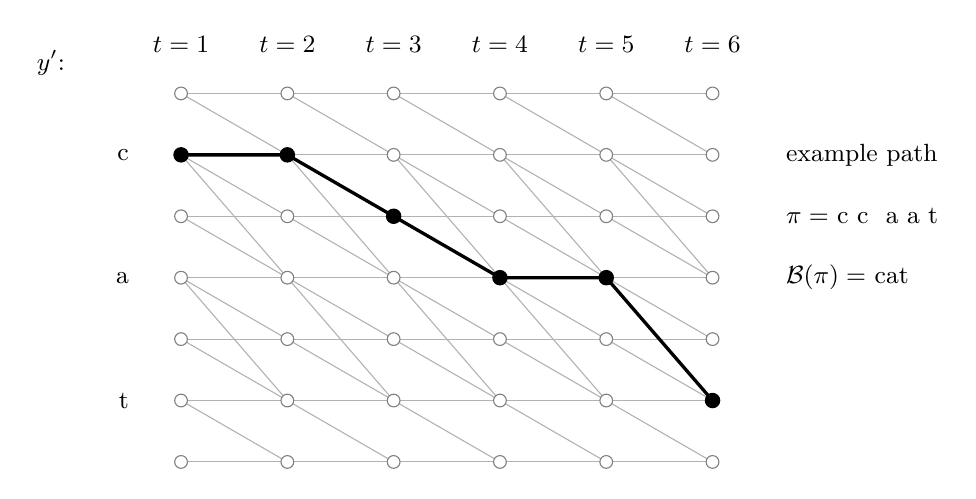
\begin{tikzpicture}[x={(1.35cm,0)},y={(0,-0.78cm)}]
\foreach \t in {1,...,5} {
  \foreach \s in {1,...,7} {\draw[gray!60] (\t,\s) -- (\t+1,\s);}
  \foreach \s in {1,...,6} {\draw[gray!60] (\t,\s) -- (\t+1,\s+1);}
  \draw[gray!60] (\t,2) -- (\t+1,4);
  \draw[gray!60] (\t,4) -- (\t+1,6);
}
\foreach \t in {1,...,6} {\foreach \s in {1,...,7} {\fill[white,draw=gray] (\t,\s) circle (2.3pt);}}
\foreach \s/\l in {1/$\varnothing$,2/c,3/$\varnothing$,4/a,5/$\varnothing$,6/t,7/$\varnothing$} {\node[font=\small,anchor=east] at (0.6,\s) {\l};}
\foreach \t in {1,...,6} {\node[font=\small,anchor=south] at (\t,0.5) {$t=\t$};}
\draw[very thick] (1,2) -- (2,2) -- (3,3) -- (4,4) -- (5,4) -- (6,6);
\foreach \t/\s in {1/2,2/2,3/3,4/4,5/4,6/6} {\fill (\t,\s) circle (2.8pt);}
\node[font=\small,anchor=west] at (6.6,2) {example path};
\node[font=\small,anchor=west] at (6.6,3) {$\pi=$ c c $\varnothing$ a a t};
\node[font=\small,anchor=west] at (6.6,4) {$\mathcal B(\pi)=$ cat};
\node[font=\small,anchor=east] at (0.0,0.5) {$y'$:};
\end{tikzpicture}
\caption{CTC lattice for the word ``cat'' with $T=6$ steps. The rows are the positions of the blank-augmented label $y'$; thin lines are the allowed transitions of Equation~\ref{eq:rec-alpha} (stay, advance, and skip over a blank between different letters). The thick path is one of the many paths that collapse to the word.}
\label{fig:rec-ctc}
\end{figure}

\paragraph{Receptive field.}
The region of the input that influences one feature is found with the recursion of Equation~\ref{eq:rec-rf}, in which $r$ is the receptive field and $j$ the distance in input pixels between adjacent features (the jump).
\begin{equation}
r_{\mathrm{out}}=r_{\mathrm{in}}+(k-1)\,j_{\mathrm{in}},\qquad j_{\mathrm{out}}=j_{\mathrm{in}}\,s.
\label{eq:rec-rf}
\end{equation}
Applied to the network (two convolutions, a pool, four convolutions, a pool, six convolutions) this gives 5, 6, 22, 24 and finally 72 pixels, so each column feature sees a $72\times72$ window, the full height of the line and about 18 time steps of context, before the recurrent layers add unbounded horizontal context.



\subsubsection{Evaluation metrics}

Accuracy is measured with the Levenshtein edit distance \cite{levenshtein1966}, the minimum number of insertions, deletions and substitutions that turn string $a$ into string $b$, computed by dynamic programming (Equation~\ref{eq:rec-lev}):
\begin{equation}
\begin{gathered}D[i][j]=\min\bigl(D[i-1][j]+1,\;D[i][j-1]+1,\;D[i-1][j-1]+\mathbb 1[a_i\ne b_j]\bigr),\\ D[i][0]=i,\ D[0][j]=j,\end{gathered}
\label{eq:rec-lev}
\end{equation}
with $d_{\mathrm{lev}}(a,b)=D[|a|][|b|]$.
For training and validation the character error rate is micro-averaged over all lines $n$ with prediction $\hat y_n$ and reference $y_n$ (Equation~\ref{eq:rec-cer}),
(equation as in the main text)
which is case-sensitive.
The end-to-end evaluation of Section~\ref{sec:results} instead averages per line the floored accuracy $\max(0,1-d_{\mathrm{lev}}(\hat y,y)/|y|)$ after converting both strings to lower case, which is slightly more lenient, so the two kinds of figure are not computed identically.
A word measure is implemented as the longest-common-subsequence (LCS) recall (Equation~\ref{eq:rec-wacc})
\begin{equation}
\mathrm{WordAcc}=\frac{\mathrm{LCS}(\text{reference words},\text{predicted words})}{\#\text{reference words}},
\label{eq:rec-wacc}
\end{equation}
which is an in-order recall and not $1-\mathrm{WER}$; a standard word error rate $\mathrm{WER}=d_{\mathrm{lev}}(\text{word sequences})/\#\text{reference words}$ was computed only once, when the public sets were re-evaluated.


\begin{figure}[h]
\centering
\begin{tikzpicture}[x=1cm,y=1cm]
\newcommand{\wcurve}[1]{\draw[#1] (0,0) .. controls (0.25,1.1) and (0.85,1.1) .. (0.7,0.45) .. controls (0.6,0.05) and (1.1,-0.05) .. (1.55,0.5);}
% column headings
\node[font=\small,align=center] at (1.0,3.25) {(a) raw crop};
\node[font=\small,align=center] at (4.2,3.25) {(b) core band};
\node[font=\small,align=center] at (7.4,3.25) {(c) skeleton};
\node[font=\small,align=center] at (10.6,3.25) {(d) re-inked};
% row A: thick, slanted
\begin{scope}[xshift=0.2cm,yshift=1.7cm,xslant=0.35]\wcurve{line width=5pt,gray!70,cap=round}\end{scope}
\begin{scope}[xshift=3.4cm,yshift=1.7cm,xslant=0.35]\wcurve{line width=5pt,gray!40,cap=round}\end{scope}
\draw[dashed] (3.3,1.55) -- (5.4,1.55) node[right,font=\scriptsize] {};
\draw[dashed] (3.3,2.35) -- (5.4,2.35);
\draw[<->] (5.2,1.55) -- (5.2,2.35); \node[font=\scriptsize,anchor=west] at (5.2,1.95) {$x_h$};
\begin{scope}[xshift=6.6cm,yshift=1.7cm,xslant=0.35]\wcurve{line width=0.8pt,black,cap=round}\end{scope}
\begin{scope}[xshift=9.8cm,yshift=1.7cm,xslant=0.35]\wcurve{line width=3pt,black,cap=round}\end{scope}
% row B: thin, upright
\begin{scope}[xshift=0.2cm,yshift=0.1cm]\wcurve{line width=1.8pt,gray!70,cap=round}\end{scope}
\begin{scope}[xshift=3.4cm,yshift=0.1cm]\wcurve{line width=1.8pt,gray!40,cap=round}\end{scope}
\draw[dashed] (3.3,-0.05) -- (5.4,-0.05);
\draw[dashed] (3.3,0.75) -- (5.4,0.75);
\draw[<->] (5.2,-0.05) -- (5.2,0.75); \node[font=\scriptsize,anchor=west] at (5.2,0.35) {$x_h$};
\begin{scope}[xshift=6.6cm,yshift=0.1cm]\wcurve{line width=0.8pt,black,cap=round}\end{scope}
\begin{scope}[xshift=9.8cm,yshift=0.1cm]\wcurve{line width=3pt,black,cap=round}\end{scope}
\node[font=\scriptsize,anchor=east] at (-0.2,2.0) {writer A};
\node[font=\scriptsize,anchor=east] at (-0.2,0.4) {writer B};
\draw[w2arr] (2.3,-0.9) -- (3.1,-0.9);
\end{tikzpicture}
\caption{Stroke normalisation of a schematic letter from two different writers. The raw strokes differ in thickness and slant (a); the core band gives the x-height $x_h$ (b); thinning reduces the stroke to a centre line (c); and the centre line is re-drawn with the width $w=\mathrm{round}(0.14\,x_h)$, identical for both writers (d). A real example is to be supplied as Figure~\ref{fig:wid-strokereal}.}
\label{fig:wid-strokenorm}
\end{figure}

\begin{itemize}
\item \emph{Skeletonisation.} The ink is thinned to a one-pixel centre line with the iterative algorithm of Zhang and Suen \cite{zhang1984}, which preserves the topology of the strokes. In each of two sub-iterations a pixel $p_1$ is deleted if the condition of Equation~\ref{eq:wid-zs} holds, namely
\begin{equation}
2\le B(p_1)\le6,\qquad A(p_1)=1,\qquad\text{and the product conditions of the sub-iteration,}
\label{eq:wid-zs}
\end{equation}
where $B(p_1)$ is the number of ink neighbours among the eight neighbours, $A(p_1)$ the number of transitions from background to ink around the ring of neighbours $P_2,\ldots,P_9$, and the product conditions are $P_2P_4P_6=0$ and $P_4P_6P_8=0$ (first sub-iteration) or $P_2P_4P_8=0$ and $P_2P_6P_8=0$ (second); the passes are repeated until no pixel changes.
\end{itemize}

\subsection{Appendix: further supporting material for Sections 3.3 to 3.5 (third condensation)}

This part of the appendix contains the staged-training diagram, the roles of the two writer classifiers, the optimisation paragraph with its equation, and the details of the text-versus-diagram clustering.

\begin{table}[h]
\centering
\fontsize{9.5}{11.5}\selectfont
\begin{tabularx}{\linewidth}{|p{3.3cm}|X|X|}
\hline
& \textbf{Ink-based classifier} & \textbf{Shape (stroke-normalised) classifier} \\
\hline
Input & Raw grey-scale line crop. & Line crop after stroke normalisation (constant pen width). \\
\hline
Used for & Real photographed pages in the classification mode. & Judging synthesised and G-code-rendered output, inside the best-of-$N$ search of Section~\ref{sec:synthesis}. \\
\hline
What was trained & All 966\,154 parameters, started from the weights of the text recogniser backbone. & Only the 13\,354 parameters of the head; the convolutional backbone is the frozen text-recogniser backbone. \\
\hline
\end{tabularx}
\caption{Roles of the two writer classifiers.}
\label{tab:wid-roles}
\end{table}

\paragraph{Optimisation.}
Both classifiers are trained with AdamW \cite{kingma2015,loshchilov2019}, which updates each parameter with a bias-corrected running mean $\hat m$ and running mean of squares $\hat v$ of the gradient and applies the weight decay separately from the gradient (Equation~\ref{eq:wid-adamw}):
\begin{equation}
\theta\leftarrow\theta-\eta\Bigl(\frac{\hat m}{\sqrt{\hat v}+\epsilon}+\lambda\theta\Bigr),\qquad\eta_t=\frac{\eta_0}{2}\Bigl(1+\cos\frac{\pi t}{T_{\max}}\Bigr),
\label{eq:wid-adamw}
\end{equation}
with weight decay $\lambda=10^{-4}$ and the cosine schedule of the learning rate $\eta_t$ over $T_{\max}$ epochs, which decreases smoothly from $\eta_0$ to zero.
Table~\ref{tab:wid-hyper} lists the settings.
The ink classifier is fully fine-tuned from the recogniser backbone, which has already learned stroke-shape features; the weights were compared and all 84 backbone tensors differ from the recogniser's.
For the shape classifier the frozen backbone (in inference mode) computes the 128-dimensional feature $f$ of every training image once, each line appearing four times (once unaugmented and three times with a different random augmentation), and only the head is trained on these 3\,680 stored vectors; all 84 backbone tensors of the stored shape model are bit-identical to those of the text recogniser.
Training only the head is fast and cannot overfit the thickness cue in the backbone, but it means that no augmentation is re-sampled between epochs.



\begin{figure}[h]
\centering
\begin{tikzpicture}[x=1cm,y=1cm]
\tikzset{sb/.style={w2box,text width=3.6cm,minimum height=1.4cm}}
\node[sb] (b) at (-5.4,0) {\textbf{1 Base}\\ own database lines, noisy labels\\ best val. loss 1.06};
\node[sb] (h) at (-0.6,0) {\textbf{2 Clean labels}\\ public line set, 6\,481 lines\\ val./test 93.87/91.60\,\%};
\node[sb] (n) at (4.5,1.2) {\textbf{3 Personal only (rejected)}\\ val./test 84.26/80.56\,\%\\ personal 90.2\,\%};
\node[sb] (j) at (4.5,-1.2) {\textbf{4 Joint, 80/20 sampler (deployed)}\\ val./test 94.03/91.82\,\%\\ personal 89.64\,\%};
\draw[w2arr] (b)--(h) node[midway,above,font=\scriptsize] {warm start};
\draw[w2arr] (h.east) -- ++(0.45,0) |- (n.west);
\draw[w2arr] (h.east) -- ++(0.45,0) |- (j.west);
\end{tikzpicture}
\caption{Staged training recipe of the text recogniser with the character accuracies (public validation and test sets, and personal validation; see Table~\ref{tab:rec-results} for the caveats).}
\label{fig:rec-stages}
\end{figure}

\paragraph{Text-versus-diagram clustering.}
A component with $\mathrm{mess}\ge0.5$, area above $0.8\wht^2$ and height above $1.2\wht$ becomes a candidate.
A candidate with a score below 0.85 is \emph{vetoed} (treated as text) when at least three text-sized neighbours stand in the same row band and the candidate is no taller than $1.9$ times the 75th percentile of their heights, which rescues large looped letters in headings.
Surviving candidates are clustered greedily by area into \texttt{MESS} blocks when their vertical gap is below $0.8\wht$ and their horizontal gap below $2\wht$, and each block receives a core box that ignores thin tails and labels.



\subsection{Appendix: further supporting material for Sections 3.3 and 3.4 (fourth condensation)}

This part of the appendix contains the full text and equations of the connected-component, skew, Gaussian-blur, batch-normalisation and staged-training passages that are summarised in Sections~\ref{sec:segmentation} and~\ref{sec:textrec}.

\subsubsection{Stage 7: connected components and the glyph-height scale}

A \emph{connected component} is a maximal set of ink pixels that touch each other.
Components are found with a run-length two-pass algorithm with union-find, a design that follows the classical sequential labelling idea \cite{rosenfeld1966} but works on runs instead of single pixels.
Each image row is first encoded as maximal runs $[s,e)$ of ink pixels.
For every pair of adjacent rows the runs are swept with two pointers, and run $i$ of the upper row and run $j$ of the lower row are merged when they touch; for 8-connectivity (diagonal neighbours count) the condition (Equation~\ref{eq:seg-adj}) is
\begin{equation}
s_i<e_j+1\ \ \wedge\ \ s_j<e_i+1,
\label{eq:seg-adj}
\end{equation}
and for 4-connectivity the $+1$ terms are dropped, where $s$ and $e$ are the start and end (exclusive) columns of the runs.
The pointer whose run ends first is advanced.
The merging uses a union-find structure with path halving \cite{tarjan1975}, roots are mapped to compact labels $1\ldots n$, and the labels are painted back run by run.
The cost is linear in the number of runs times an almost constant factor, which is far cheaper than a pixel-wise method for thin handwriting strokes.
For every component the area, bounding box and centroid are computed by sorting the labelled pixels by label.

The \emph{glyph height} $\wht$ is estimated from the components themselves, as given in Equation~\ref{eq:seg-ht}.
Heights of components with area at least 30 pixels and width below $12$ times the height (which excludes rules and long underlines) are collected; $h_{\mathrm{med}}$ is their median, and
\begin{equation}
\wht=\mathrm{median}\bigl\{h_c:\;0.3\,h_{\mathrm{med}}<h_c<3\,h_{\mathrm{med}}\bigr\},
\label{eq:seg-ht}
\end{equation}
where $h_c$ is the height of component $c$ (the default is 30 pixels if no component qualifies).
Because the cleaning stages change the component set, $\wht$ is computed three times: after the first binarisation (for the recovery stage), after faint filtering (for edge, column and rule removal), and finally on the cleaned set (for grouping and rendering).


\subsubsection{Stage 5: skew estimation and rotation}

If the text lines are tilted, row-based grouping and the recogniser both degrade.
The tilt of the page is estimated by the classical projection-profile principle: when the lines are horizontal, the row-sum profile of the ink has sharp peaks (line bodies) and deep troughs (gaps between lines), and any tilt smears them (Figure~\ref{fig:seg-skew}).
For a candidate angle $\theta$ the ink mask, reduced by a factor 4 (any ink in a $4\times4$ block), is rotated by nearest-neighbour sampling, the row profile $P_\theta(y)=\sum_xR_\theta(y,x)$ is formed, and the score is its variance (Equation~\ref{eq:seg-skew})
\begin{equation}
J(\theta)=\mathrm{Var}_y\bigl[P_\theta(y)\bigr],\qquad \theta^*=\arg\max_\theta J(\theta),
\label{eq:seg-skew}
\end{equation}
where $R_\theta$ is the rotated reduced mask and $\mathrm{Var}_y$ the variance over rows.
The search uses a coarse grid $\theta\in\{-r,-r+0.5,\ldots,r\}$ of 33 angles for $r=8^\circ$ followed by a fine grid $\theta^*\pm0.5^\circ$ in steps of $0.1^\circ$, so the angular resolution is $0.1^\circ$ and only 44 rotations of a mask of one sixteenth of the original area are needed.
Rotation about the image centre $(c_x,c_y)=((W-1)/2,(H-1)/2)$ uses inverse mapping with bilinear interpolation (nearest neighbour for masks):
\begin{equation}
\begin{pmatrix}x_s\\y_s\end{pmatrix}=\begin{pmatrix}\cos\theta&-\sin\theta\\ \sin\theta&\cos\theta\end{pmatrix}\begin{pmatrix}x-c_x\\y-c_y\end{pmatrix}+\begin{pmatrix}c_x\\c_y\end{pmatrix},
\label{eq:seg-rot}
\end{equation}
in which $(x,y)$ is an output pixel and $(x_s,y_s)$ the source position that is sampled; outside samples are filled with 255 for the colour page and 0 for masks.
The page is rotated only if $|\theta^*|\ge0.15^\circ$; stages 3 and 4 (grey conversion, correction, binarisation, speckle removal) are then recomputed on the rotated image, and a second residual pass with range $\pm3^\circ$ follows.


A single global angle is estimated, so page curl and keystone are not corrected; the objective was preferred to a Hough transform because ruled lines and diagrams dominate edge directions. A sign mismatch between rotation and scoring that doubled the skew in an early version was corrected.


\paragraph{Gaussian blur from three box blurs.}
A Gaussian blur with standard deviation $\sigma$ is approximated by three successive box means of equal radius $r$, because the repeated convolution of a uniform kernel converges to a Gaussian shape by the central-limit argument.
A single box of full width $w=2r+1$ has the variance $(w^2-1)/12$, and three independent passes add their variances to
\begin{equation}
\sigma_{\mathrm{real}}^2=\frac{w^2-1}{4},\qquad w=2r+1,\qquad r=\max\Bigl(1,\;\mathrm{round}\Bigl(\tfrac12\sqrt{\tfrac{4\sigma^2}{3}+1}\Bigr)\Bigr),
\label{eq:seg-gauss}
\end{equation}
where the radius $r$ is the one chosen by the implementation for a requested nominal scale $\sigma$.
An evaluation of Equation~\ref{eq:seg-gauss} shows that the box width produced by this rounding is approximately $\sqrt{4\sigma^2/3+1}+1$, so that $\sigma_{\mathrm{real}}\approx\sigma/\sqrt3\approx0.58\,\sigma$.
For example, a nominal scale $\sigma=60$ (the illumination blur for a page 1800 pixels wide) gives $r=35$, $w=71$ and $\sigma_{\mathrm{real}}=\sqrt{(71^2-1)/4}\approx35.5$, and a nominal scale of 9.5 gives $r=6$ and $\sigma_{\mathrm{real}}\approx6.5$.
The nominal $\sigma$ in this report is therefore a \emph{blur scale parameter} and not the realised standard deviation, and all constants of the block were tuned with the implementation as it stands.


\paragraph{Staged recipe.}
Training was carried out in four stages (Table~\ref{tab:rec-stages}, Figure~\ref{fig:rec-stages}), and each stage is motivated by a limitation that was found in the previous one.
\begin{enumerate}
\item \emph{Base stage.} The published recipe was reproduced on lines that were segmented from database pages by the student's own tools. The data turned out to be small and noisy because of the labelling defect and segmentation errors, and the best validation loss was 1.06.
\item \emph{Clean-label stage.} The network was warm-started from the base stage and trained on the public line-level IAM set, whose human-checked labels remove all segmentation and labelling noise.
\item \emph{Personal fine-tuning (rejected).} Fine-tuning on the personal lines alone raised the accuracy on the personal validation lines but reduced the accuracy on the general data by about ten points (catastrophic forgetting, Table~\ref{tab:rec-forget}); freezing the convolutional layers reduced the forgetting only slightly.
\item \emph{Joint stage (deployed).} Training continues from the clean-label stage on both data sets at once, with a weighted sampler: each public line receives the weight $w_T=(1-f)/n_T$ and each personal line $w_P=f/n_P$, where $n_T=6\,481$, $n_P\approx280$ and $f=0.20$, and $n_T$ indices are drawn per epoch with replacement with probability proportional to the weights (Equation~\ref{eq:rec-sampler}),
\begin{equation}
P(i)=\frac{w_i}{\sum_jw_j}.
\label{eq:rec-sampler}
\end{equation}
In expectation 20\,\% of every epoch ($\approx1\,296$ draws) is taken from the personal set, so that each personal line is seen about 4.6 times per epoch with fresh random augmentation, and 80\,\% from the public set. The checkpoint of the epoch with the largest $\min(\text{accuracy}_{\mathrm{public}},\text{accuracy}_{\mathrm{personal}})$ is kept, so that neither domain is sacrificed.
\end{enumerate}



A sweep over learning rate, LSTM width, depth, convolution width, dropout and optimiser (14 configurations of 50 epochs) was programmed, but no result file was kept, so the deployed architecture is the published one and not an optimum found by the student.
Training was done offline on a general-purpose computer; the training log of the joint stage was not kept, so epoch-by-epoch curves cannot be shown, and the stored joint checkpoint contains weights only.


\paragraph{Batch normalisation.}
Deep networks train poorly if the distribution of each layer's inputs keeps changing, so every convolution is followed by batch normalisation \cite{ioffe2015}.
During training, for each channel the mean $\mu_B$ and variance $\sigma_B^2$ are computed over the mini-batch and all spatial positions, and the output (Equation~\ref{eq:rec-bn}) is
\begin{equation}
\hat x=\frac{x-\mu_B}{\sqrt{\sigma_B^2+\varepsilon}},\qquad y=\gamma\hat x+\beta,\qquad\varepsilon=10^{-5},
\label{eq:rec-bn}
\end{equation}
where $\gamma$ and $\beta$ are learned scale and shift parameters of the channel.
Running averages of the mean and variance are kept during training, and at test time they replace $\mu_B$ and $\sigma_B^2$, which turns the layer into the fixed per-channel affine map $y=a\,x+b$ with
\begin{equation}
a=\frac{\gamma}{\sqrt{\sigma^2_{\mathrm{run}}+\varepsilon}},\qquad b=\beta-a\,\mu_{\mathrm{run}},
\label{eq:rec-bnfold}
\end{equation}
where $\mu_{\mathrm{run}}$ and $\sigma^2_{\mathrm{run}}$ are the running statistics; this is exactly the form that the inference implementation uses.


\subsection{Appendix: label generation for the database pages}

The labels of the database pages were produced by reading the printed prompt of each form and aligning its word list with the detected ink word runs by dynamic programming; the alignment cost for a run of measured width $a$ and an expected width $e$ is $c(a,e)=((a-e)/(e+1))^2$, with a penalty of 0.5 for the merging or splitting of words.
